\section{Verse-Space Seq2Seq RNN}

One of the possible causes of failure encountered in the previous models could be related to the way the original text was partitioned.
In fact, up to the last networks, we developed them to predict one single token given a fixed-length sample of the previous ones, meaning that in the majority of cases we were trying to predict a token in the middle of a verse (thus, having very little information about the rhyming scheme) from a sample starting from a random position inside another verse.
Also, as we generally used a \texttt{step length} grater than one in order both to reduce the computational cost and to avoid overfitting, some of the markers and the tokens at the end of the verse (i.e. those being more useful to understand both the structure and the rhyming scheme) were not used neither for training nor for validating, going "wasted".

\begin{figure}[!htb]
    \centering
    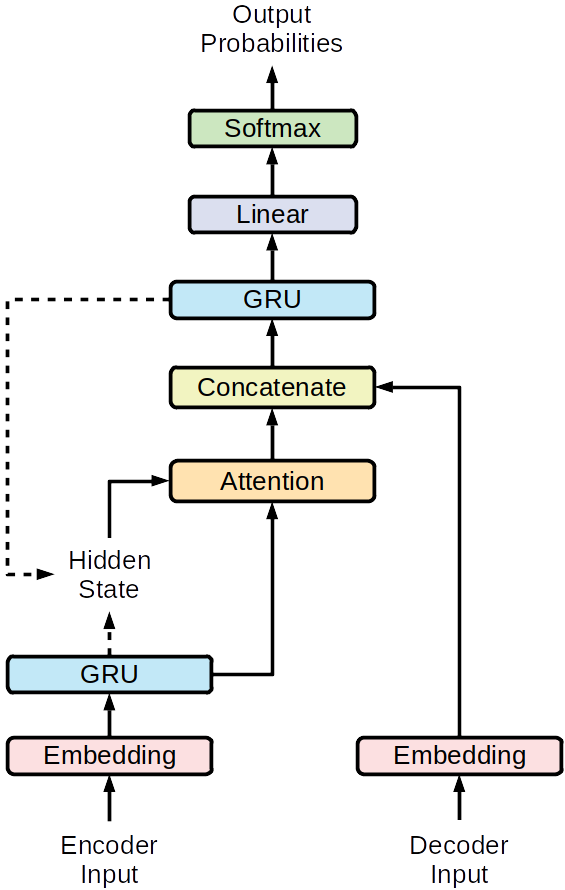
\includegraphics[scale=0.65]{images/model-3.png}%
    \caption{Seq2Seq RNN Architecture}%
    \label{seq2seq}
\end{figure}

Therefore, with the aim of overcoming this structural problem, we tried to use a \textit{Sequence To Sequence} model for \textit{Neural Machine Translation}, also involving attention mechanisms because of the great complexity of the text.
Even though these kind of models are generally used to translate from one natural language to another, we wanted to apply the same idea to the \textit{Divine Comedy}, trying to "translate" a sample of verses into the entire, following verse, and we decided to fix the number of verses, i.e. our new \texttt{sequence lenght}, to three, as from the previous three verses (included the one having as a single token the \texttt{=tercet=} marker) the network should be able to understand both the structure and the rhyming scheme, namely it should be able to understand whether the next verse should contain a \texttt{=tercet=} marker or not, and if not how to properly end the verse so that it rhymes when necessary.

An important thing to be noticed is that, given that the verse to be predicted is the $i_{th}$ one and the input patch is made up of the verses $i-3$ to $i-1$, initially we used as output sequence the output verse only (or rather, the $i_{th}$ verse).
This, however, gave terrible results, in line with the fact that, as well as previous architectures, the network could not understand the inner patterns of the text.
Taking that in mind, we decided at first to use as output a sample of the last three verses (from the $i-2_{th}$ to the $i_{th}$) and, finally, to use all of the four verses as output, because even though the two ways gave almost similar results, in this last case it was easier to perform the prediction/generation phase, as the input sequence had to be entirely passed both to the encoder and to the decoder in order to get as output the last verse only.

Finally, as it can be seen from the picture \ref{seq2seq}, this model is composed of two different, interconnected modules, that are:
\begin{itemize}
    \item an \texttt{\textsc{Encoder}}, made up of an \textsc{Embedding} and a \textsc{GRU} layer, which takes the input sample and returns both the output and the hidden state of the \textsc{GRU}
    \item a \texttt{\textsc{Decoder}}, made up of an \textsc{Embedding} and a \textsc{GRU} layer as well as an \textsc{Attention} layer, which takes the latest decoded token as input, the latest hidden state\footnote{
        During the first iteration, these are the \textit{start token} and the hidden state of the encoder.
    } and the output of the encoder, and returns the hidden state of the \textsc{GRU} and the output processed through a \textsc{Dense} layer
\end{itemize}

As the output returned from this architecture is the vector of probabilities for a single token, we had to develop a custom training loop that repeatedly called the model using the new output (and the new hidden state as well) as inputs until the \textit{end token} of the output sequence was predicted.
This, clearly, led to a more costly training.

\subsubsection{\textsc{Hyperparameters and Results}}

This time, the hyperparameters were:
\begin{itemize}
    \item the dimension of the \textsc{Embedding} layer
    \item the number of units of the \textsc{GRU} layer
    \item the kind of \textsc{Attention} layer, which could be either:
    \begin{itemize}
        \item Additive, or \textit{Bahdanau-style} \parencite{bahdanau2014neural}
        \item Multiplicative, or \textit{Luong-style} \parencite{luong2015effective}
    \end{itemize}
    \item the dropout rate for the \textsc{RNN} layers
\end{itemize}

The main problem of both the variations (\textit{Word-Level} and \textit{Subword-Level}) of this architecture is that, as we said, the training cost was too expensive, with some configuration needing up to twenty minutes per epoch.
This, combined with the fact that the convergence was really slow (looking at the loss/accuracy plots, we saw that the trend was clearly increasing in performances without reaching a plateau, but still this increase was linear and very slight), did not allow us to get great results.
Indeed, the few configurations that were able to achieve results which were greater than the previous two models, did not score well in the \texttt{ngrams plagiarism test}, as they were in fact copying the original verses from the \textit{Divine Comedy}, therefore we decided to abandon the idea of using \textit{RNNs} and exploit, instead, new \textit{state-of-the-art} models for \textit{Neural Machine Translation}. 